\providecommand{\Fun}{\operatorname{Fun}}
\providecommand{\Cat}{\mathcal{C}at}
\providecommand{\QCat}{\mathcal{Q}\mathcal{C}at}
\providecommand{\sSet}{s\mathcal{S}et}
\providecommand{\qcOne}{\mathbf{1}}   %
\providecommand{\colim}{\operatorname{colim}\nolimits}
\providecommand{\qcTwo}{\mathbf{2}}   %
\providecommand{\CospanShape}{\lrcorner}   %

\section{\trLimit{}与\trColimit}\label{sec:limits-and-colimits}

我们现在来引入在某个\trInfinityCosmos{}中取值于一个\trInfinityCategory{} $A$
\emph{之内}的\trDiagram{}的\trLimit{}与\trColimit{}。我们考虑两种\trDiagram{}：
\begin{itemize}
\item 由单纯集 $J$ 索引、并在一个一般的\trInfinityCosmos{}中取值于一个%
\trInfinityCategory{} $A$ 的\trDiagram{}；以及
\item 由一个\trInfinityCategory{} $J$ 索引、并在一个\trCartesianClosed{}%
\trInfinityCosmos{}中取值于一个\trInfinityCategory{} $A$ 的\trDiagram{}。%
\footnote{对于例 1.2.24 中由 $(\infty,1)$-\trCategory{}构成的那些\trInfinityCosmos{}%
而言，这些概念之间没有本质差别：在 $\QCat$ 中二者同义反复地相同；而在所有与之%
\trBiequivalence{}的\trInfinityCosmos{}中，由\trInfinityCategory{} $J$ 索引%
\trDiagram{}的\trInfinityCategory{}，与把其\trUnderlyingQuasiCategory{}视作一个%
\trSimplicialSet{}来索引\trDiagram{}的\trInfinityCategory{}二者\trEquivalence{}
（见命题 10.3.5）。}
\end{itemize}

\begin{definition}[图表]\label{def:diagram}
所谓\trInfinityCategory{} $A$ 中形状为 $J$ 的一个\textbf{\trDiagram}（diagram），
是指某个\trDiagram{}∞-\trCategory{}的一个\trElement{} $d\colon 1\to A^J$。%
\footnote{当 $A^J$ 是某个\trCartesianClosed{}\trInfinityCosmos{}中的指数时，
\trDiagram{}与\trFunctor{} $d\colon J\to A$ 一一对应。}
这里索引形状 $J$ 或者是一个\trSimplicialSet——此时对包含 $A$ 的任何%
\trInfinityCosmos{} $\mathcal{K}$，$A^J$ 均有定义——或者是一个%
\trInfinityCategory——此时对包含 $A$ 的任何\trCartesianClosed{}%
\trInfinityCosmos{} $\mathcal{K}$，$A^J$ 均有定义。
$J$-索引\trDiagram{}之间的一个态射是\trInfinityCategory{} $A^J$ 中的
一个态射。
\end{definition}

在\trInfinityCosmos{} $\mathcal{K}$ 中构造\trDiagram{}∞-\trCategory{}的两种方式
都定义出\trSimplicial{}双\trFunctor
\begin{equation*}
\sSet^{\mathrm{op}}\times\mathcal{K}\longrightarrow\mathcal{K}
\qquad\qquad
\mathcal{K}^{\mathrm{op}}\times\mathcal{K}\longrightarrow\mathcal{K}
\end{equation*}
\begin{equation*}
(J,A)\longmapsto A^J
\qquad\qquad
(J,A)\longmapsto A^J
\end{equation*}
在两种索引语境中，都存在\trTerminal{}对象 $1$，使得对每个\trInfinityCategory{} $A$
都有 $A^1\cong A$。沿唯一映射 $!\colon J\to 1$ 作限制，便诱导出%
\trConstantFunctor{} $\Delta\colon A\to A^J$。

对于由单纯集索引的\trDiagram{}∞-\trCategory{}与由另一个\trInfinityCategory{}索引的%
\trDiagram{}∞-\trCategory{}，我们有意混用二者的记号，因为我们在第一部分中就前一种
情形证明的所有结果，同样适用于后一种情形。为行文简洁起见，在本节余下部分中我们只
谈及由单纯集索引的\trDiagram{}。

\begin{definition}[\trLimit{}与\trColimit{}函子]\label{def:limit-colimit}
一个\trInfinityCategory{} $A$ \textbf{具备形状 $J$ 的一切\trColimit}（admits all
colimits of shape $J$），如果\trConstantFunctor{} $\Delta\colon A\to A^J$ 容许
一个\trLeftAdjoint{}；而 $A$ \textbf{具备形状 $J$ 的一切\trLimit}（admits all
limits of shape $J$），如果该\trConstantFunctor{}容许一个\trRightAdjoint{}：
\begin{center}
\begin{tikzpicture}[x=1.4em,y=1.4em]
  \node (AJ) at (0,0) {$A^J$};
  \node (A) at (5.4,0) {$A$};
  \draw[->] (1.0,0.66) to[bend left=22] node[above]{$\colim$} (4.4,0.66);
  \node at (2.1,0.30) {$\dashv$};
  \draw[->] (4.4,0) -- (1.0,0);
  \node at (3.4,0.26) {$\Delta$};
  \node at (2.1,-0.30) {$\dashv$};
  \draw[->] (1.0,-0.66) to[bend left=22] node[below]{$\lim$} (4.4,-0.66);
\end{tikzpicture}
\end{center}
在由\trCategory{}组成的\trInfinityCosmos{}中，
\cref{def:limit-colimit}化归为经典定义的\trLimit{}与\trColimit{}函子；
但在一般的\trInfinityCategory{}中，\trLimit{}与\trColimit{}应视作与
经典概念「同伦\trLimit{}」「同伦\trColimit{}」相类比的对象。
在某些情形，这一对应可以精确化：每个\trQuasiCategory{}都%
\trEquivalence{}于某个\trKanComplex\trEnrichedCategory{}的同伦相干\trNerve
\cite[7.2.2]{bib111}，而\trKanComplex\trEnrichedCategory{}中的同伦\trLimit\trCone{}或
同伦\trColimit\trCone{}，恰对应于同伦相干\trNerve{}中的\trLimit\trCone{}或\trColimit\trCone
（见 Lurie 的\cite[4.2.4.1]{bib78}或\cite[6.1.4, 6.2.7]{bib113}）。
在\trInfinityCategory{}的语境中，没有更严格意义的\trLimit{}或%
\trColimit{}概念，所以「同伦」一词通常省去。
\end{definition}

以集合 $J$ 为索引的\trDiagram{}——即索引形状是由集合 $J$ 索引的%
\trTerminal{}对象 $1$ 的\trCoproduct{}的情形——的\trLimit{}或\trColimit{}，
分别称为\trProduct{}或\trCoproduct{}。

\begin{lemma}\label{lem:products-homotopy-category}
\trInfinityCategory{} $A$ 中的\trProduct{}或\trCoproduct{}，也定义出其\trHomotopyCategory{}
$\mathrm{h}A$ 中的\trProduct{}或\trCoproduct{}。
\end{lemma}
\begin{proof}
当 $J$ 是集合时，\trDiagram{}∞-\trCategory{}本身分解为由 $J$ 索引的
$A$ 的副本的\trProduct

\begin{equation*}
A^J\cong\prod_{j\in J}A
\end{equation*}
由于把\trInfinityCategory{}送到其\trHomotopyCategory{}的%
\trTwoFunctor{}
\begin{equation*}
\begin{gathered}
\mathrm{h}\mathcal{K}
\xrightarrow{\ \mathrm{h}\Fun(1,-)\ }\Cat\\
A\longmapsto\mathrm{h}A
\end{gathered}
\end{equation*}
保持\trProduct{}，故当 $J$ 为集合时有 $\mathrm{h}(A^J)\cong\mathrm{h}(\prod_{j\in J}A)\cong\prod_{j\in J}\mathrm{h}A\cong(\mathrm{h}A)^J$。于是，在这一特殊情形，
\cref{def:limit-colimit}中定义\trInfinityCategory{}里的\trProduct{}或\trCoproduct{}的那些%
\trAdjunction{}，便下降为定义其\trHomotopyCategory{}中\trProduct{}或\trCoproduct{}的%
\trAdjunction{}：
\begin{equation*}
\mbox{\begin{tikzpicture}[x=1.4em,y=1.4em]
  \node (hAJ) at (0,0) {$(\mathrm{h}A)^J\cong\mathrm{h}(A^J)$};
  \node (hA) at (7.6,0) {$\mathrm{h}A$};
  \draw[->] (3.3,0.66) to[bend left=22] node[above]{$\colim$} (6.5,0.66);
  \node at (4.4,0.30) {$\dashv$};
  \draw[->] (6.5,0) -- (3.3,0);
  \node at (5.6,0.26) {$\Delta$};
  \node at (4.4,-0.30) {$\dashv$};
  \draw[->] (3.3,-0.66) to[bend left=22] node[below]{$\lim$} (6.5,-0.66);
\end{tikzpicture}}
\end{equation*}
这在 $J=\emptyset$ 的情形依然成立，正解释了\cref{eq:initial-terminal-homotopy-category}中
的观察。
\end{proof}

\begin{warning}\label{war:converse-false}
这一论证并不能推广到更一般的\trLimit{}或\trColimit{}概念，而且%
∞-\trCategory{}中的这类\trLimit{}或\trColimit{}通常并不下降为%
\trHomotopyCategory{}中的\trLimit{}或\trColimit{}。%
\footnote{这类行为在抽象同伦论中是人们熟悉的：同伦\trLimit{}与%
同伦\trColimit{}一般并不是\trHomotopyCategory{}中的\trLimit{}或%
\trColimit{}。}在 §3.2 中，我们将观察到\trHomotopyCategory{}构造%
未能保持更复杂的\trCotensor{}，即便在 $J=\qcTwo$ 这一相对简单的情形中亦然。
\end{warning}

\cref{def:limit-colimit}的问题在于它不够一般：许多\trInfinityCategory{}%
对特定索引形状的\trDiagram{}有某些、但非全部的\trLimit{}。因此，
值得把\cref{def:limit-colimit}重新表述成一种使我们能考虑单个\trDiagram{}
$d\colon 1\to A^J$ 或一族\trDiagram{}之\trLimit{}的形式。为此，
我们利用下面这个 2-\trCategory{}式的概念，它 op-对偶化了更为人熟知的
绝对（\trKanExtension）图。

\begin{definition}[绝对左\trLifting]\label{def:absolute-left-lifting}
在 2-\trCategory{}中给定形如 $C\xrightarrow{g}A\xleftarrow{f}B$ 的图，%
$g$ 沿 $f$ 的一个%
\emph{绝对左\trLifting}（absolute left lifting）由一个 1-\trCell{}
$\ell\colon C\to B$ 及一个 2-\trCell{} $\lambda\colon g\Rightarrow f\ell$
构成，如下左图所示，
使得任何如下中图所示的 2-\trCell{}都能唯一地经由 $(\ell,\lambda)$
分解成如下右图所示的形状：
\begin{center}
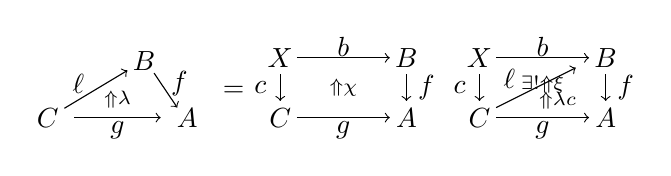
\begin{tikzpicture}[x=1.2em,y=1.2em]
  \node (C1) at (0,0) {$C$};
  \node (A1) at (4.2,0) {$A$};
  \node (B1) at (2.9,1.7) {$B$};
  \draw[->] (0.5,0.28) -- (2.4,1.42);
  \node at (0.92,1.02) {$\ell$};
  \draw[->] (3.2,1.34) -- (3.9,0.3);
  \node at (3.96,1.02) {$f$};
  \draw[->] (0.8,0) -- (3.4,0);
  \node at (2.1,-0.38) {$g$};
  \node at (2.1,0.55) {$\scriptstyle\Uparrow\lambda$};
  \node at (5.6,0.8) {$=$};
  \node (X2) at (7.0,1.8) {$X$};
  \node (B2) at (10.8,1.8) {$B$};
  \node (C2) at (7.0,0) {$C$};
  \node (A2) at (10.8,0) {$A$};
  \draw[->] (7.5,1.8) -- (10.3,1.8);
  \node at (8.9,2.14) {$b$};
  \draw[->] (10.8,1.3) -- (10.8,0.5);
  \node at (11.4,0.9) {$f$};
  \draw[->] (7.0,1.3) -- (7.0,0.5);
  \node at (6.4,0.9) {$c$};
  \draw[->] (7.5,0) -- (10.3,0);
  \node at (8.9,-0.38) {$g$};
  \node at (8.9,0.9) {$\scriptstyle\Uparrow\chi$};
  \node (X3) at (13.0,1.8) {$X$};
  \node (B3) at (16.8,1.8) {$B$};
  \node (C3) at (13.0,0) {$C$};
  \node (A3) at (16.8,0) {$A$};
  \draw[->] (13.5,1.8) -- (16.3,1.8);
  \node at (14.9,2.14) {$b$};
  \draw[->] (16.8,1.3) -- (16.8,0.5);
  \node at (17.4,0.9) {$f$};
  \draw[->] (13.0,1.3) -- (13.0,0.5);
  \node at (12.4,0.9) {$c$};
  \draw[->] (13.5,0) -- (16.3,0);
  \node at (14.9,-0.38) {$g$};
  \draw[->] (13.5,0.3) -- (15.9,1.5);
  \node at (13.9,1.16) {$\ell$};
  \node at (14.9,1.0) {$\scriptstyle\exists!\Uparrow\xi$};
  \node at (15.35,0.5) {$\scriptstyle\Uparrow\lambda c$};
\end{tikzpicture}
\end{center}
对偶地，在 2-\trCategory{}中，$g$ 沿 $f$ 的一个\emph{绝对右\trLifting}（absolute
right lifting）
由一个 1-\trCell{} $r\colon C\to B$ 及一个 2-\trCell{}
$\rho\colon fr\Rightarrow g$ 构成，如下左图所示，
使得任何如下中图所示的 2-\trCell{}都能唯一地经由 $(r,\rho)$
分解成如下右图所示的形状：
\begin{center}
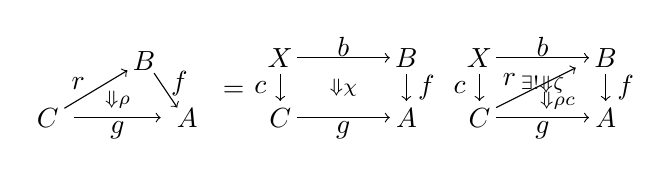
\begin{tikzpicture}[x=1.2em,y=1.2em]
  \node (C1) at (0,0) {$C$};
  \node (A1) at (4.2,0) {$A$};
  \node (B1) at (2.9,1.7) {$B$};
  \draw[->] (0.5,0.28) -- (2.4,1.42);
  \node at (0.92,1.02) {$r$};
  \draw[->] (3.2,1.34) -- (3.9,0.3);
  \node at (3.96,1.02) {$f$};
  \draw[->] (0.8,0) -- (3.4,0);
  \node at (2.1,-0.38) {$g$};
  \node at (2.1,0.55) {$\scriptstyle\Downarrow\rho$};
  \node at (5.6,0.8) {$=$};
  \node (X2) at (7.0,1.8) {$X$};
  \node (B2) at (10.8,1.8) {$B$};
  \node (C2) at (7.0,0) {$C$};
  \node (A2) at (10.8,0) {$A$};
  \draw[->] (7.5,1.8) -- (10.3,1.8);
  \node at (8.9,2.14) {$b$};
  \draw[->] (10.8,1.3) -- (10.8,0.5);
  \node at (11.4,0.9) {$f$};
  \draw[->] (7.0,1.3) -- (7.0,0.5);
  \node at (6.4,0.9) {$c$};
  \draw[->] (7.5,0) -- (10.3,0);
  \node at (8.9,-0.38) {$g$};
  \node at (8.9,0.9) {$\scriptstyle\Downarrow\chi$};
  \node (X3) at (13.0,1.8) {$X$};
  \node (B3) at (16.8,1.8) {$B$};
  \node (C3) at (13.0,0) {$C$};
  \node (A3) at (16.8,0) {$A$};
  \draw[->] (13.5,1.8) -- (16.3,1.8);
  \node at (14.9,2.14) {$b$};
  \draw[->] (16.8,1.3) -- (16.8,0.5);
  \node at (17.4,0.9) {$f$};
  \draw[->] (13.0,1.3) -- (13.0,0.5);
  \node at (12.4,0.9) {$c$};
  \draw[->] (13.5,0) -- (16.3,0);
  \node at (14.9,-0.38) {$g$};
  \draw[->] (13.5,0.3) -- (15.9,1.5);
  \node at (13.9,1.16) {$r$};
  \node at (14.9,1.0) {$\scriptstyle\exists!\Downarrow\zeta$};
  \node at (15.35,0.5) {$\scriptstyle\Downarrow\rho c$};
\end{tikzpicture}
\end{center}
\end{definition}

当这些\trLifting{}存在时，左\trLifting{}与右\trLifting{}分别定义出复合\trFunctor
$f_{\ast}\colon\mathrm{h}\Fun(C,B)\to\mathrm{h}\Fun(C,A)$
的\trLeftAdjoint{}与\trRightAdjoint{}，
而其 2-\trCell{}分别给出这些\trAdjunction{}的\trUnit{}与\trCounit{}%
在对象 $g$ 处的分量。「绝对」这一形容词指的是如下的稳定性。

\begin{lemma}\label{lem:absolute-lifting-restriction}
绝对左\trLifting{}图与绝对右\trLifting{}图在其定义域对象的限制下稳定：
若 $(\ell,\lambda)$ 定义了 $g$ 沿 $f$ 的一个绝对左\trLifting{}，
则对任何 $c\colon X\to C$，限制偶 $(\ell c,\lambda c)$ 定义了
$gc$ 沿 $f$ 的一个绝对左\trLifting{}。
\begin{center}
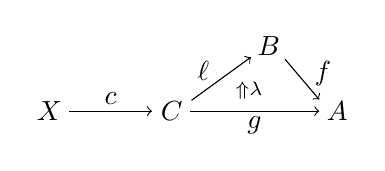
\begin{tikzpicture}[x=1.3em,y=1.3em]
  \node (X) at (0,0) {$X$};
  \node (C) at (3.4,0) {$C$};
  \node (A) at (8.0,0) {$A$};
  \node (B) at (6.1,1.8) {$B$};
  \draw[->] (0.55,0) -- (2.85,0);
  \node at (1.7,0.34) {$c$};
  \draw[->] (3.95,0.3) -- (5.6,1.5);
  \node at (4.28,1.12) {$\ell$};
  \draw[->] (6.55,1.44) -- (7.5,0.32);
  \node at (7.6,1.04) {$f$};
  \draw[->] (3.9,0) -- (7.5,0);
  \node at (5.7,-0.38) {$g$};
  \node at (5.55,0.58) {$\scriptstyle\Uparrow\lambda$};
\end{tikzpicture}
\end{center}
\end{lemma}

\begin{proof}
\cref{lem:absolute-lifting-restriction}的证明是\cref{ex:restriction-absolute-lifting}。
\end{proof}

\trAdjunction{}的\trUnit{}与\trCounit{}分别给出绝对左\trLifting{}图与绝对
右\trLifting{}图的重要例子：

\begin{lemma}\label{lem:unit-counit-absolute-liftings}
一个 2-\trCell{} $\eta\colon\mathrm{id}_B\Rightarrow uf$ 定义某个%
\trAdjunction{} $f\dashv u$ 的\trUnit{}，当且仅当 $(f,\eta)$ 定义一个
绝对左\trLifting{}图：
\begin{center}
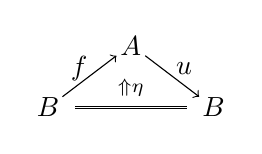
\begin{tikzpicture}[x=1.3em,y=1.3em]
  \node (B1) at (0,0) {$B$};
  \node (B2) at (4.6,0) {$B$};
  \node (T1) at (2.3,1.7) {$A$};
  \draw[->] (0.4,0.3) -- (1.9,1.44);
  \node at (0.86,1.08) {$f$};
  \draw[->] (2.7,1.44) -- (4.2,0.3);
  \node at (3.78,1.08) {$u$};
  \draw[double] (0.75,0) -- (3.85,0);
  \node at (2.3,0.55) {$\scriptstyle\Uparrow\eta$};
\end{tikzpicture}
\end{center}
对偶地，一个 2-\trCell{} $\epsilon\colon fu\Rightarrow\mathrm{id}_A$ 定义
某个\trAdjunction{}的\trCounit{}，当且仅当 $(u,\epsilon)$ 定义一个绝对
右提升图表：
\begin{center}
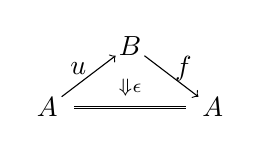
\begin{tikzpicture}[x=1.3em,y=1.3em]
  \node (A1) at (0,0) {$A$};
  \node (A2) at (4.6,0) {$A$};
  \node (T1) at (2.3,1.7) {$B$};
  \draw[->] (0.4,0.3) -- (1.9,1.44);
  \node at (0.86,1.08) {$u$};
  \draw[->] (2.7,1.44) -- (4.2,0.3);
  \node at (3.78,1.08) {$f$};
  \draw[double] (0.75,0) -- (3.85,0);
  \node at (2.3,0.55) {$\scriptstyle\Downarrow\epsilon$};
\end{tikzpicture}
\end{center}
\end{lemma}

\begin{proof}
绝对右\trLifting{}图
\begin{center}
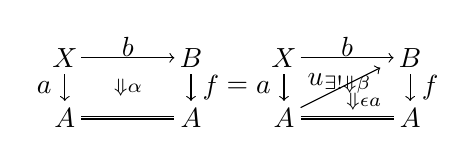
\begin{tikzpicture}[x=1.2em,y=1.2em]
  \node (X1) at (0,1.8) {$X$};
  \node (B1) at (3.8,1.8) {$B$};
  \node (A1) at (0,0) {$A$};
  \node (A2) at (3.8,0) {$A$};
  \draw[->] (0.5,1.8) -- (3.3,1.8);
  \node at (1.9,2.14) {$b$};
  \draw[->] (3.8,1.3) -- (3.8,0.5);
  \node at (4.4,0.9) {$f$};
  \draw[->] (0,1.3) -- (0,0.5);
  \node at (-0.62,0.9) {$a$};
  \draw[double] (0.5,0) -- (3.3,0);
  \node at (1.9,0.9) {$\scriptstyle\Downarrow\alpha$};
  \node at (5.2,0.9) {$=$};
  \node (X2) at (6.6,1.8) {$X$};
  \node (B2) at (10.4,1.8) {$B$};
  \node (A3) at (6.6,0) {$A$};
  \node (A4) at (10.4,0) {$A$};
  \draw[->] (7.1,1.8) -- (9.9,1.8);
  \node at (8.5,2.14) {$b$};
  \draw[->] (10.4,1.3) -- (10.4,0.5);
  \node at (11.0,0.9) {$f$};
  \draw[->] (6.6,1.3) -- (6.6,0.5);
  \node at (5.98,0.9) {$a$};
  \draw[double] (7.1,0) -- (9.9,0);
  \draw[->] (7.1,0.3) -- (9.5,1.5);
  \node at (7.55,1.14) {$u$};
  \node at (8.5,1.0) {$\scriptstyle\exists!\Downarrow\beta$};
  \node at (9.0,0.48) {$\scriptstyle\Downarrow\epsilon a$};
\end{tikzpicture}
\end{center}
的泛性质断言：每个\trNaturalTransformation{}
$\alpha\colon fb\Rightarrow a$ 都有跨同伦 2-\trCategory{}的诸%
\trHomCategory{}之间\trAdjunction{}的唯一转置
$\beta\colon b\Rightarrow ua$：
\begin{center}
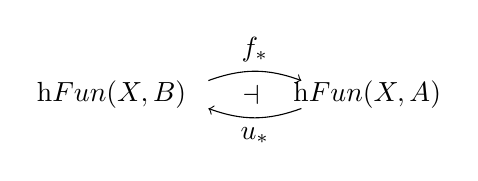
\begin{tikzpicture}[x=1.4em,y=1.4em]
  \node (HB) at (0,0) {$\mathrm{h}\Fun(X,B)$};
  \node (HA) at (6.6,0) {$\mathrm{h}\Fun(X,A)$};
  \draw[->] (2.5,0.36) to[bend left=20] node[above]{$f_{\ast}$} (4.9,0.36);
  \node at (3.6,0) {$\dashv$};
  \draw[->] (4.9,-0.36) to[bend left=20] node[below]{$u_{\ast}$} (2.5,-0.36);
\end{tikzpicture}
\end{center}
于是，若 $f\dashv u$ 带有余单位 $\epsilon$，则\cref{prop:adjunction-preservation}(ii)
便给出这条诱导的\trAdjunction{}，而 $(u,\epsilon)$ 定义 $\mathrm{id}_A$ 沿 $f$
的一个绝对右\trLifting{}。
反过来，一个\trAdjunction{}的\trUnit{}与三角等式可以从绝对右\trLifting{}图的%
\trUniversalProperty{}中提取出来。细节留作\cref{ex:pasting-reproves-unit-counit}。
\end{proof}

特别地，\cref{def:limit-colimit}中\trAdjunction{} $\colim\dashv\Delta\dashv\lim$
的\trUnit{}与\trCounit{}定义出绝对左\trLifting{}图与绝对右\trLifting{}图：
\begin{center}
\begin{tikzpicture}[x=1.3em,y=1.3em]
  \node (AJ1) at (0,0) {$A^{J}$};
  \node (T1) at (2.9,1.7) {$A$};
  \node (AJ2) at (5.8,0) {$A^{J}$};
  \draw[->] (0.45,0.3) -- (2.45,1.42);
  \node at (0.95,1.1) {$\colim$};
  \draw[->] (3.35,1.42) -- (5.35,0.3);
  \node at (4.95,1.1) {$\Delta$};
  \draw[double] (0.75,0) -- (5.05,0);
  \node at (2.9,0.55) {$\scriptstyle\Uparrow\eta$};
  \node at (8.2,0.8) {与};
  \node (AJ3) at (10.6,0) {$A^{J}$};
  \node (T2) at (13.5,1.7) {$A$};
  \node (AJ4) at (16.4,0) {$A^{J}$};
  \draw[->] (11.05,0.3) -- (13.05,1.42);
  \node at (11.62,1.1) {$\lim$};
  \draw[->] (13.95,1.42) -- (15.95,0.3);
  \node at (16.5,1.1) {$\Delta$};
  \draw[double] (11.35,0) -- (15.65,0);
  \node at (13.5,0.55) {$\scriptstyle\Downarrow\epsilon$};
\end{tikzpicture}
\end{center}
由\cref{lem:absolute-lifting-restriction}，这些泛性质在限制到%
\trDiagram{}∞-\trCategory{}的任何\trSubobject{}时依然保持。这激发了如下定义：

\begin{definition}[\trLimit{}与\trColimit]\label{def:limit-colimit-cones}
\trInfinityCategory{} $A$ 中形状为 $J$ 的一族\trDiagram{}
$d\colon D\to A^J$ 的一个\textbf{\trColimit}（colimit）由一个绝对左\trLifting{}图
\begin{center}
\begin{tikzpicture}[x=1.3em,y=1.3em]
  \node (D) at (0,0) {$D$};
  \node (T) at (2.9,1.7) {$A$};
  \node (R) at (5.8,0) {$A^J$};
  \draw[->] (0.45,0.3) -- (2.45,1.42);
  \node at (0.95,1.1) {$\colim d$};
  \draw[->] (3.35,1.42) -- (5.35,0.3);
  \node at (4.9,1.1) {$\Delta$};
  \draw[->] (0.75,0) -- (5.05,0);
  \node at (2.9,-0.38) {$d$};
  \node at (2.9,0.55) {$\scriptstyle\Uparrow\eta$};
\end{tikzpicture}
\end{center}
给出，它由一个\trGeneralizedElement{} $\colim d\colon D\to A$ 连同一个%
\trColimit\trCone $\eta\colon d\Rightarrow\Delta\colim d$ 构成。

对偶地，\trInfinityCategory{} $A$ 中形状为 $J$ 的一族\trDiagram{}
$d\colon D\to A^J$ 的一个\textbf{\trLimit}（limit）由一个绝对右\trLifting{}图
\begin{center}
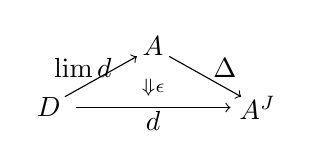
\begin{tikzpicture}[x=1.3em,y=1.3em]
  \node (D) at (0,0) {$D$};
  \node (T) at (2.9,1.7) {$A$};
  \node (R) at (5.8,0) {$A^J$};
  \draw[->] (0.45,0.3) -- (2.45,1.42);
  \node at (0.95,1.1) {$\lim d$};
  \draw[->] (3.35,1.42) -- (5.35,0.3);
  \node at (4.9,1.1) {$\Delta$};
  \draw[->] (0.75,0) -- (5.05,0);
  \node at (2.9,-0.38) {$d$};
  \node at (2.9,0.55) {$\scriptstyle\Downarrow\epsilon$};
\end{tikzpicture}
\end{center}
给出，它由一个\trGeneralizedElement{} $\lim d\colon D\to A$ 连同一个%
\trLimit\trCone $\epsilon\colon\Delta\lim d\Rightarrow d$ 构成。
\end{definition}

\begin{remark}\label{rem:families-of-diagrams}
若 $A$ 具有 $J$ 形状的所有\trLimit{}，则\cref{lem:absolute-lifting-restriction}
蕴含：任何\trDiagram{}族 $d\colon D\to A^J$ 都有\trLimit{}，它由把\trLimit{}%
函子 $\lim\colon A^J\to A$ 与 $d$ 复合而定义。在一个由 $(\infty,1)$-\trCategory{}%
构成的\trInfinityCosmos{}中，若每个\trDiagram{} $d\colon 1\to A^J$ 都有%
\trLimit{}，则 $A$ 具有 $J$ 形状的所有\trLimit{}（见推论 12.2.10）；
但在一般情形，\trDiagram{}族无法化归为单个\trDiagram{}。
\end{remark}

\begin{example}[\trInitial{}\trElement{}是\trEmptyDiagram{}的\trColimit]%
\label{exa:initial-colimit-empty}
一个\trInitial{}\trElement{}定义任意\trInfinityCategory{} $A$ 中形状
$\emptyset$ 的\trEmptyDiagram{}的一个\trColimit{}。由 $A$ 中空图表构成的%
\trInfinityCategory{} $A^{\emptyset}\simeq\qcOne$ 是\trTerminal{}的，%
故\trConstantFunctor{}化为 $!\colon A\to 1$。
要证明\trInitial{}\trElement{}是\cref{def:limit-colimit-cones}意义上的%
\trColimit{}，我们必须验证：一个\trInitial{}\trElement{}定义一个%
2-\trCell{}为恒同的绝对左\trLifting{}图
\begin{center}
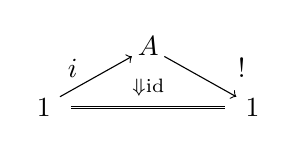
\begin{tikzpicture}[x=1.3em,y=1.3em]
  \node (One) at (0,0) {$1$};
  \node (A) at (2.9,1.7) {$A$};
  \node (OneR) at (5.8,0) {$1$};
  \draw[->] (0.45,0.3) -- (2.45,1.42);
  \node at (0.8,1.1) {$i$};
  \draw[->] (3.35,1.42) -- (5.35,0.3);
  \node at (5.5,1.1) {$!$};
  \draw[double] (0.75,0) -- (5.05,0);
  \node at (2.9,0.55) {$\scriptstyle\Downarrow\mathrm{id}$};
\end{tikzpicture}
\end{center}
\begin{center}
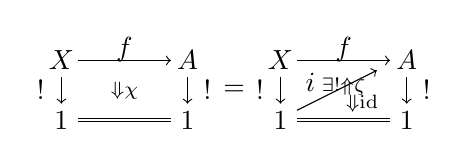
\begin{tikzpicture}[x=1.2em,y=1.2em]
  \node (X1) at (0,1.8) {$X$};
  \node (A1) at (3.8,1.8) {$A$};
  \node (O1) at (0,0) {$1$};
  \node (O2) at (3.8,0) {$1$};
  \draw[->] (0.5,1.8) -- (3.3,1.8);
  \node at (1.9,2.14) {$f$};
  \draw[->] (3.8,1.3) -- (3.8,0.5);
  \node at (4.4,0.9) {$!$};
  \draw[->] (0,1.3) -- (0,0.5);
  \node at (-0.62,0.9) {$!$};
  \draw[double] (0.5,0) -- (3.3,0);
  \node at (1.9,0.9) {$\scriptstyle\Downarrow\chi$};
  \node at (5.2,0.9) {$=$};
  \node (X2) at (6.6,1.8) {$X$};
  \node (A2) at (10.4,1.8) {$A$};
  \node (O3) at (6.6,0) {$1$};
  \node (O4) at (10.4,0) {$1$};
  \draw[->] (7.1,1.8) -- (9.9,1.8);
  \node at (8.5,2.14) {$f$};
  \draw[->] (10.4,1.3) -- (10.4,0.5);
  \node at (11.0,0.9) {$!$};
  \draw[->] (6.6,1.3) -- (6.6,0.5);
  \node at (5.98,0.9) {$!$};
  \draw[double] (7.1,0) -- (9.9,0);
  \draw[->] (7.1,0.3) -- (9.5,1.5);
  \node at (7.5,1.14) {$i$};
  \node at (8.5,1.0) {$\scriptstyle\exists!\Uparrow\zeta$};
  \node at (9.05,0.5) {$\scriptstyle\Downarrow\mathrm{id}$};
\end{tikzpicture}
\end{center}
由于∞-\trCategory{} $1$ 是\trTwoTerminalObject{}，居于上面方图中的
2-\trCell{} $\chi$ 是唯一的，即恒同。于是，该绝对左\trLifting{}图的泛性质
断言：对任何 $f\colon X\to A$，存在唯一的 2-\trCell{}
$\zeta\colon i!\Rightarrow f$——恰如\cref{lem:initial-element-universal-property}
所给出者。
\end{example}

\begin{example}[\trInitial{}\trElement{}是恒同\trFunctor{}的\trLimit]%
\label{exa:initial-limit-identity}
在\trCartesianClosed{}\trInfinityCosmos{}中，\trInitial{}\trElement{}
$i\colon 1\to A$ 还可以看作恒同\trFunctor{} $\mathrm{id}_A\colon A\to A$
的一个\trLimit{}。\footnote{这一结果在命题 9.4.10 中推广到非\trCartesianClosed{}
\trInfinityCosmos{}。%
}\trAdjunction{} $i\dashv !$ 的\trCounit{}
$\epsilon\colon i!\Rightarrow\mathrm{id}_A$ 跨命题 1.4.5 的 2-\trAdjunction{}
$A\times-\dashv(-)^{A}$ 转置，定义出下左图所示的\trLimit\trCone
\begin{center}
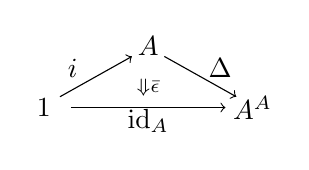
\begin{tikzpicture}[x=1.3em,y=1.3em]
  \node (One) at (0,0) {$1$};
  \node (A) at (2.9,1.7) {$A$};
  \node (AA) at (5.8,0) {$A^{A}$};
  \draw[->] (0.45,0.3) -- (2.45,1.42);
  \node at (0.8,1.1) {$i$};
  \draw[->] (3.35,1.42) -- (5.35,0.3);
  \node at (4.9,1.1) {$\Delta$};
  \draw[->] (0.75,0) -- (5.05,0);
  \node at (2.9,-0.38) {$\mathrm{id}_A$};
  \node at (2.9,0.55) {$\scriptstyle\Downarrow\bar\epsilon$};
\end{tikzpicture}
\end{center}
其绝对性（从而其泛性质）可验证如下。对任何 $f\colon X\to A$，须证每个
2-\trCell{} $\chi\colon\Delta f\Rightarrow(\mathrm{id}_A)!$——即以 $f$
为顶点、覆盖该\trDiagram{}的一个\trCone——都通过唯一的
$\zeta\colon f\Rightarrow i!$ 而分解：
\begin{center}
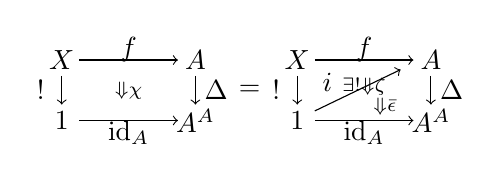
\begin{tikzpicture}[x=1.15em,y=1.15em]
  \node (X1) at (0,1.9) {$X$};
  \node (A1) at (4.2,1.9) {$A$};
  \node (O1) at (0,0) {$1$};
  \node (AA1) at (4.2,0) {$A^{A}$};
  \draw[->] (0.55,1.9) -- (3.65,1.9);
  \node at (2.1,2.24) {$f$};
  \draw[->] (4.2,1.4) -- (4.2,0.5);
  \node at (4.85,0.95) {$\Delta$};
  \draw[->] (0,1.4) -- (0,0.5);
  \node at (-0.66,0.95) {$!$};
  \draw[->] (0.55,0) -- (3.65,0);
  \node at (2.1,-0.4) {$\mathrm{id}_A$};
  \node at (2.1,0.95) {$\scriptstyle\Downarrow\chi$};
  \node at (5.9,0.95) {$=$};
  \node (X2) at (7.4,1.9) {$X$};
  \node (A2) at (11.6,1.9) {$A$};
  \node (O2) at (7.4,0) {$1$};
  \node (AA2) at (11.6,0) {$A^{A}$};
  \draw[->] (7.95,1.9) -- (11.05,1.9);
  \node at (9.5,2.24) {$f$};
  \draw[->] (11.6,1.4) -- (11.6,0.5);
  \node at (12.25,0.95) {$\Delta$};
  \draw[->] (7.4,1.4) -- (7.4,0.5);
  \node at (6.74,0.95) {$!$};
  \draw[->] (7.95,0) -- (11.05,0);
  \node at (9.5,-0.4) {$\mathrm{id}_A$};
  \draw[->] (7.95,0.3) -- (10.65,1.6);
  \node at (8.35,1.2) {$i$};
  \node at (9.5,1.05) {$\scriptstyle\exists!\Downarrow\zeta$};
  \node at (10.15,0.45) {$\scriptstyle\Downarrow\bar\epsilon$};
\end{tikzpicture}
\end{center}
这一泛性质最容易通过再次跨 2-\trAdjunction{} $A\times-\dashv(-)^{A}$
转置来验证\yizhu{$\hat\chi$ 恒指 $\chi$ 的转置。}；此时我们必须建立
粘贴等式
\begin{rveq}\label{eq:ex2311-pasting}
\mbox{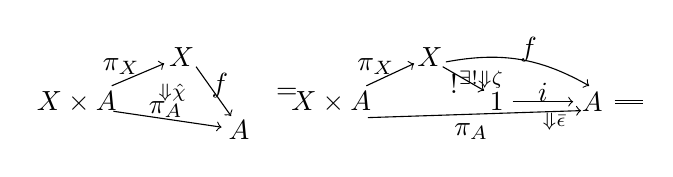
\begin{tikzpicture}[x=1.15em,y=1.15em]
  \node (XA1) at (0,0.9) {$X\times A$};
  \node (X1) at (3.3,2.3) {$X$};
  \node (A1) at (5.1,0) {$A$};
  \draw[->] (1.1,1.4) -- (2.75,2.1);
  \node at (1.4,2.0) {$\pi_X$};
  \draw[->] (3.75,2.0) -- (4.85,0.45);
  \node at (4.5,1.4) {$f$};
  \draw[->] (1.15,0.6) -- (4.55,0.1);
  \node at (2.8,0.66) {$\pi_A$};
  \node at (3.0,1.2) {$\scriptstyle\Downarrow\hat\chi$};
  \node at (6.6,1.15) {$=$};
  \node (XA2) at (8.0,0.9) {$X\times A$};
  \node (X2) at (11.1,2.3) {$X$};
  \node (One) at (13.2,0.9) {$1$};
  \node (A2) at (16.2,0.9) {$A$};
  \draw[->] (9.1,1.4) -- (10.6,2.1);
  \node at (9.4,2.0) {$\pi_X$};
  \draw[->] (11.6,2.15) to[bend left=20] (16.1,1.4);
  \node at (14.2,2.55) {$f$};
  \draw[->] (11.5,2.0) -- (12.8,1.25);
  \node at (11.85,1.45) {$!$};
  \draw[->] (13.7,0.9) -- (15.6,0.9);
  \node at (14.65,1.18) {$i$};
  \draw[->] (9.15,0.4) -- (15.85,0.62);
  \node at (12.4,-0.05) {$\pi_A$};
  \node at (12.7,1.6) {$\scriptstyle\exists!\Downarrow\zeta$};
  \node at (15.0,0.28) {$\scriptstyle\Downarrow\bar\epsilon$};
  \draw[double] (16.9,0.9) -- (17.8,0.9);
\end{tikzpicture}}
\end{rveq}
注意，把\cref{eq:ex2311-pasting}的右端沿函子
$\mathrm{id}_X\times i\colon X\cong X\times 1\to X\times A$ 限制，就回收了
2-\trCell{} $\zeta$，因为 $\bar\epsilon i=\mathrm{id}_i$。这告诉我们：
给定 $\chi$，我们必须把 2-\trCell{} $\zeta\colon f\Rightarrow i!$ 定义为
$\hat\chi$ 沿函子 $\mathrm{id}_X\times i\colon X\to X\times A$ 的限制。
由 $\zeta$ 的这一定义与笛卡尔积的 \trTwoFunctor{}性——它告诉我们
$\epsilon\pi_A=\pi_A(X\times\epsilon)$——可得
\begin{center}
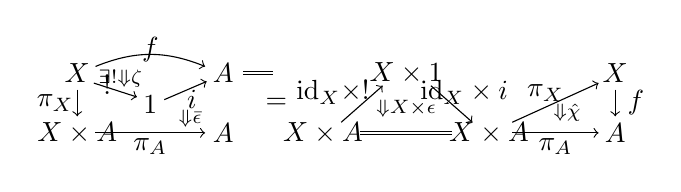
\begin{tikzpicture}[x=1.2em,y=1.2em]
  \node (X1) at (0,1.8) {$X$};
  \node (A1) at (4.4,1.8) {$A$};
  \node (O1) at (2.2,0.85) {$1$};
  \node (XA1) at (0,0) {$X\times A$};
  \node (A2) at (4.4,0) {$A$};
  \draw[->] (0.55,2.0) to[bend left=22] (3.85,2.0);
  \node at (2.2,2.52) {$f$};
  \draw[->] (0,1.3) -- (0,0.5);
  \node at (-0.66,0.9) {$\pi_X$};
  \draw[->] (0.5,1.5) -- (1.8,1.08);
  \node at (0.9,1.46) {$!$};
  \draw[->] (2.62,1.0) -- (3.9,1.55);
  \node at (3.45,1.02) {$i$};
  \draw[->] (0.55,0) -- (3.85,0);
  \node at (2.2,-0.4) {$\pi_A$};
  \node at (1.3,1.62) {$\scriptstyle\exists!\Downarrow\zeta$};
  \node at (3.4,0.42) {$\scriptstyle\Downarrow\bar\epsilon$};
  \draw[double] (5.0,1.8) -- (5.9,1.8);
  \node at (6.0,0.9) {$=$};
  \node (XA3) at (7.4,0) {$X\times A$};
  \node (XO) at (9.9,1.8) {$X\times 1$};
  \node (XA4) at (12.4,0) {$X\times A$};
  \node (X2) at (16.2,1.8) {$X$};
  \node (A3) at (16.2,0) {$A$};
  \draw[double] (8.5,0) -- (11.3,0);
  \draw[->] (7.95,0.32) -- (9.2,1.42);
  \node at (7.7,1.22) {$\mathrm{id}_X\times !$};
  \draw[->] (10.65,1.42) -- (11.9,0.32);
  \node at (11.65,1.22) {$\mathrm{id}_X\times i$};
  \node at (9.9,0.72) {$\scriptstyle\Downarrow X\times\epsilon$};
  \draw[->] (13.1,0.32) -- (15.7,1.5);
  \node at (14.1,1.2) {$\pi_X$};
  \draw[->] (16.2,1.3) -- (16.2,0.5);
  \node at (16.82,0.9) {$f$};
  \draw[->] (13.1,0) -- (15.7,0);
  \node at (14.4,-0.4) {$\pi_A$};
  \node at (14.75,0.62) {$\scriptstyle\Downarrow\hat\chi$};
\end{tikzpicture}
\end{center}
由「\trWhiskering{}的自然性」（见附录 B 中的\cref{lem:naturality-of-whiskering}），右端的粘贴复合可以求值为
$\pi_X(X\times\epsilon)$ 继以 $\hat\chi$ 的竖直复合，而
$\pi_X(X\times\epsilon)$ 是恒同 2-\trCell{}，故该复合就是 $\hat\chi$。
这就验证了所要的粘贴等式\cref{eq:ex2311-pasting}。
\end{example}

∞-\trCategory{}中的某些\trLimit{}与\trColimit{}因形式上的理由而存在。例如，
一条抽象的 2-\trCategory{}式引理使得同伦论中的一项经典结果得以有一个
形式化的证明，该结果计算「可裂」\trSimplicialObject{}的诸\trColimit{}，
这些\trColimit{}通常称作\trGeometricRealization{}。在证明这一点之前，
我们先引入所涉及的索引形状。

\begin{definition}[\trSplit{}\trAugmented{}（余）\trSimplicialObject]\label{def:split-augmented}
在定义 1.1.1 中引入的、由有限非空序数与保序映射组成的\trSimplexCategory{}
$\Delta$，构成由有限序数与保序映射组成的\trCategory{} $\Delta_{+}$ 的
全子范畴，
后者自由地添入空序数 $[-1]$ 作为\trInitial{}对象。\trCategory{} $\Delta_{+}$
又构成\trCategory{}
$\Delta_{\perp}$ 的宽子范畴，后者在每一对相邻序数之间添入一枚「额外的」
\trDegeneracyOperator{} $\sigma^{-1}\colon[n+1]\twoheadrightarrow[n]$，包括
$\sigma^{-1}\colon[0]\twoheadrightarrow[-1]$。\trCategory{} $\Delta_{+}$ 还构成\trCategory{}
$\Delta_{\top}$
的宽子范畴，后者在每一对相邻序数之间于另一侧添入一枚「额外的」
\trDegeneracyOperator{} $\sigma^{n+1}\colon[n+1]\twoheadrightarrow[n]$，包括 $\sigma^{0}\colon[0]\twoheadrightarrow[-1]$。
范畴 $\Delta_{\perp}$ 与 $\Delta_{\top}$ 还可以按另一种方式来描述：存在从它们到
$\Delta$ 中的忠实嵌入，其在对象上的作用为 $[n]\mapsto[n+1]$，并把 $\Delta_{\perp}$
与 $\Delta_{\top}$ 分别等同于有限非空序数与保序映射中保持底元素或保持顶元素者
所构成的子范畴。以 $\Delta\subset\Delta_{+}\subset\Delta_{\perp},\Delta_{\top}$
为索引的共变\trDiagram{}分别称为\textbf{\trCosimplicialObject}（cosimplicial
objects）、\textbf{余增广\trCosimplicialObject}（coaugmented cosimplicial
objects）与\textbf{\trSplit{}余增广\trCosimplicialObject}（split coaugmented
cosimplicial objects）（无论对 $\Delta_{\perp}$ 还是对 $\Delta_{\top}$ 而言）；
而反变\trDiagram{}则分别称为\textbf{\trSimplicialObject}（simplicial objects）、%
\textbf{\trAugmented{}\trSimplicialObject}（augmented simplicial objects）与%
\textbf{\trSplit{}\trAugmented{}\trSimplicialObject}（split augmented simplicial
objects）。当需要消歧 $\Delta_{\perp}$ 与 $\Delta_{\top}$ 时，我们把前一个范畴
称作一种「底部可裂」（bottom splitting），把后一个范畴称作一种「顶部可裂」
（top splitting），但这一术语并非标准。

\trInfinityCategory{} $A$ 中的一个\trCosimplicialObject{} $d\colon 1\to A^{\Delta}$
\textbf{容许一个余增广}（admits a coaugmentation）或\textbf{容许一个裂分}（admits
a splitting），如果它沿诸限制\trFunctor{}提升
\begin{center}
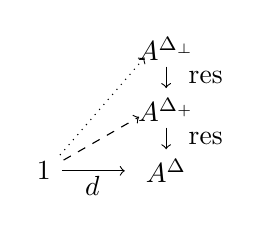
\begin{tikzpicture}[x=1.3em,y=1.3em]
  \node (Atop) at (3.4,3.4) {$A^{\Delta_{\perp}}$};
  \node (Amid) at (3.4,1.7) {$A^{\Delta_{+}}$};
  \node (Abot) at (3.4,0) {$A^{\Delta}$};
  \node (One) at (0,0) {$1$};
  \draw[->] (3.4,2.9) -- (3.4,2.3);
  \node at (4.5,2.6) {$\mathrm{res}$};
  \draw[->] (3.4,1.2) -- (3.4,0.6);
  \node at (4.5,0.9) {$\mathrm{res}$};
  \draw[->] (0.5,0) -- (2.25,0);
  \node at (1.35,-0.42) {$d$};
  \draw[->,dashed] (0.55,0.3) -- (2.65,1.5);
  \draw[->,dotted] (0.45,0.44) -- (2.8,3.15);
\end{tikzpicture}
\end{center}
而在顶部可裂的情形中，$\Delta_{\perp}$ 被替换为 $\Delta_{\top}$。容许余增广与
裂分的\trCosimplicialObject{}之族，由\trGeneralizedElement{}
$\mathrm{res}\colon A^{\Delta_{\perp}}\twoheadrightarrow A^{\Delta}$ 展示。
\end{definition}

在任何\trAugmented{}\trCosimplicialObject{}中，其底\trCosimplicialObject{}上都存在
一个\trCone{}，其顶点由在 $[-1]\in\Delta_{+}$ 处取值而得。这个\trCone{}由把
唯一的\trNaturalTransformation{}
\begin{rveq}\label{eq:nu-initial-transformation}
\mbox{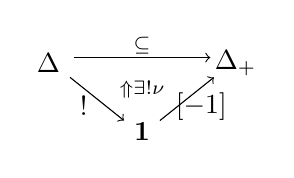
\begin{tikzpicture}[x=1.3em,y=1.3em]
  \node (D) at (0,0) {$\Delta$};
  \node (Dp) at (5.2,0) {$\Delta_{+}$};
  \node (One) at (2.6,-1.9) {$\qcOne$};
  \draw[->] (0.7,0.15) -- (4.5,0.15);
  \node at (2.6,0.49) {$\scriptstyle\subseteq$};
  \draw[->] (0.6,-0.4) -- (2.1,-1.6);
  \node at (0.98,-1.2) {$!$};
  \draw[->] (3.1,-1.6) -- (4.6,-0.4);
  \node at (4.25,-1.2) {$[-1]$};
  \node at (2.6,-0.75) {$\scriptstyle\Uparrow\exists!\nu$};
\end{tikzpicture}}
\end{rveq}
与 $A$ 作余张量而定义；这一\trNaturalTransformation{}之所以存在，是因为
$[-1]\colon\qcOne\to\Delta_{+}$ 是\trInitial{}对象（见\cref{lem:initial-element-universal-property}）。

\begin{proposition}[\trTotalization{}/\trGeometricRealization]\label{prop:split-limits}
设 $A$ 为任一\trInfinityCategory{}。$A$ 中每个容许余增广与裂分的%
\trCosimplicialObject{}都有一个\trLimit{}，其\trLimit\trCone{}由余增广定义；
对偶地，$A$ 中每个容许增广与裂分的\trSimplicialObject{}都有一个%
\trColimit{}，其\trColimit\trCone{}由增广定义。也就是说，存在绝对的
右\trLifting{}图与左\trLifting{}图
\begin{center}
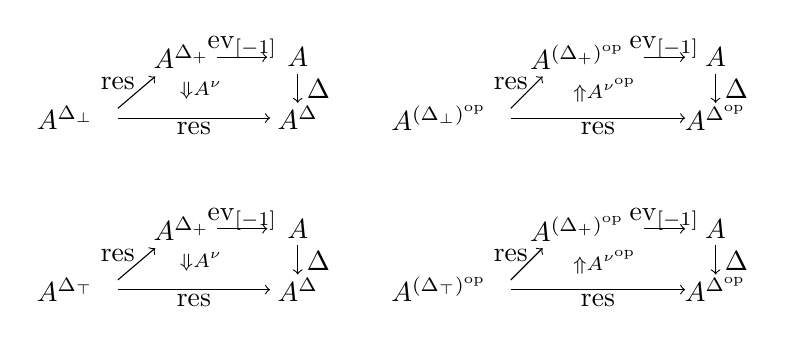
\begin{tikzpicture}[x=1.0em,y=1.0em]
  \node (B1) at (0,0) {$A^{\Delta_{\perp}}$};
  \node (T1) at (4.2,2.2) {$A^{\Delta_{+}}$};
  \node (T1R) at (8.4,2.2) {$A$};
  \node (R1) at (8.4,0) {$A^{\Delta}$};
  \draw[->] (1.9,0.35) -- (3.25,1.5);
  \node at (1.9,1.25) {$\mathrm{res}$};
  \draw[->] (5.5,2.2) -- (7.3,2.2);
  \node at (6.4,2.54) {$\mathrm{ev}_{[-1]}$};
  \draw[->] (8.4,1.6) -- (8.4,0.55);
  \node at (9.15,1.05) {$\Delta$};
  \draw[->] (1.9,0) -- (7.4,0);
  \node at (4.65,-0.38) {$\mathrm{res}$};
  \node at (4.9,1.0) {$\scriptstyle\Downarrow A^{\nu}$};
  \node (B2) at (13.5,0) {$A^{(\Delta_{\perp})^{\mathrm{op}}}$};
  \node (T2) at (18.5,2.2) {$A^{(\Delta_{+})^{\mathrm{op}}}$};
  \node (T2R) at (23.5,2.2) {$A$};
  \node (R2) at (23.5,0) {$A^{\Delta^{\mathrm{op}}}$};
  \draw[->] (16.1,0.35) -- (17.25,1.5);
  \node at (16.1,1.25) {$\mathrm{res}$};
  \draw[->] (20.9,2.2) -- (22.4,2.2);
  \node at (21.65,2.54) {$\mathrm{ev}_{[-1]}$};
  \draw[->] (23.5,1.6) -- (23.5,0.55);
  \node at (24.25,1.05) {$\Delta$};
  \draw[->] (16.1,0) -- (22.4,0);
  \node at (19.25,-0.38) {$\mathrm{res}$};
  \node at (19.5,1.0) {$\scriptstyle\Uparrow A^{\nu^{\mathrm{op}}}$};
  \node (B3) at (0,-6.2) {$A^{\Delta_{\top}}$};
  \node (T3) at (4.2,-4.0) {$A^{\Delta_{+}}$};
  \node (T3R) at (8.4,-4.0) {$A$};
  \node (R3) at (8.4,-6.2) {$A^{\Delta}$};
  \draw[->] (1.9,-5.85) -- (3.25,-4.7);
  \node at (1.9,-4.95) {$\mathrm{res}$};
  \draw[->] (5.5,-4.0) -- (7.3,-4.0);
  \node at (6.4,-3.66) {$\mathrm{ev}_{[-1]}$};
  \draw[->] (8.4,-4.6) -- (8.4,-5.65);
  \node at (9.15,-5.15) {$\Delta$};
  \draw[->] (1.9,-6.2) -- (7.4,-6.2);
  \node at (4.65,-6.58) {$\mathrm{res}$};
  \node at (4.9,-5.2) {$\scriptstyle\Downarrow A^{\nu}$};
  \node (B4) at (13.5,-6.2) {$A^{(\Delta_{\top})^{\mathrm{op}}}$};
  \node (T4) at (18.5,-4.0) {$A^{(\Delta_{+})^{\mathrm{op}}}$};
  \node (T4R) at (23.5,-4.0) {$A$};
  \node (R4) at (23.5,-6.2) {$A^{\Delta^{\mathrm{op}}}$};
  \draw[->] (16.1,-5.85) -- (17.25,-4.7);
  \node at (16.1,-4.95) {$\mathrm{res}$};
  \draw[->] (20.9,-4.0) -- (22.4,-4.0);
  \node at (21.65,-3.66) {$\mathrm{ev}_{[-1]}$};
  \draw[->] (23.5,-4.6) -- (23.5,-5.65);
  \node at (24.25,-5.15) {$\Delta$};
  \draw[->] (16.1,-6.2) -- (22.4,-6.2);
  \node at (19.25,-6.58) {$\mathrm{res}$};
  \node at (19.5,-5.2) {$\scriptstyle\Uparrow A^{\nu^{\mathrm{op}}}$};
\end{tikzpicture}
\end{center}
其中的 2-\trCell{}都是由把\cref{eq:nu-initial-transformation}与 $A$ 作
余张量、再作限制而得的。而且，这样的\trLimit{}与\trColimit{}是绝对的：
被\trInfinityCategory{}之间的任何\trFunctor{} $f\colon A\to B$ 保持。
\end{proposition}

\begin{proof}
由附录 B 中的\cref{exa:delta-adjoint-diagram}，包含\trFunctor{} $\Delta\hookrightarrow\Delta_{\perp}$ 容许一个%
\trRightAdjoint{}；由于 $\qcOne$ 在 $\Cat$ 中是\trTwoTerminalObject{}，这个%
\trAdjunction{}自动可以视为「在 $\qcOne$ 之上」的\trAdjunction{}。
\trInitial{}\trElement{} $[-1]\in\Delta_{+}\subset\Delta_{\perp}$ 定义了到%
\trConstantFunctor{}的一个\trLeftAdjoint{}：
\begin{center}
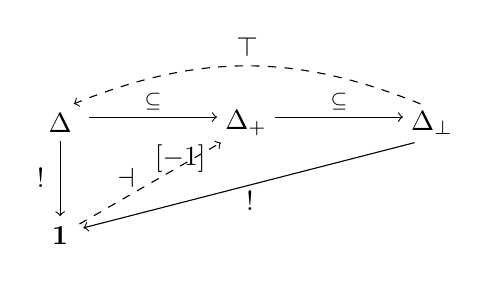
\begin{tikzpicture}[x=1.4em,y=1.4em]
  \node (D) at (0,0) {$\Delta$};
  \node (Dp) at (4.8,0) {$\Delta_{+}$};
  \node (Dperp) at (9.6,0) {$\Delta_{\perp}$};
  \draw[->] (0.75,0.16) -- (4.05,0.16);
  \node at (2.4,0.56) {$\scriptstyle\subseteq$};
  \draw[->] (5.55,0.16) -- (8.85,0.16);
  \node at (7.2,0.56) {$\scriptstyle\subseteq$};
  \draw[->,dashed] (9.3,0.5) to[bend right=22] node[above]{$\top$} (0.35,0.5);
  \node (One) at (0,-2.9) {$\qcOne$};
  \draw[->] (0,-0.45) -- (0,-2.4);
  \node at (-0.5,-1.4) {$!$};
  \draw[->,dashed] (0.5,-2.6) -- (4.15,-0.5);
  \node at (3.1,-0.9) {$[-1]$};
  \node at (1.7,-1.4) {$\dashv$};
  \draw[->] (9.15,-0.5) -- (0.6,-2.7);
  \node at (4.9,-2.0) {$!$};
\end{tikzpicture}
\end{center}
而该\trAdjunction{}的\trCounit{}沿包含
$\Delta\subset\Delta_{+}\subset\Delta_{\perp}$ 的限制，恰为%
\cref{eq:nu-initial-transformation}的 2-\trCell{}。对\trInfinityCosmos{}
$\mathcal{K}$ 中的任何\trInfinityCategory{} $A$，这些\trAdjunction{}都被%
\trTwoFunctor{} $A^{(-)}\colon\Cat^{\mathrm{op}}\to\mathrm{h}\mathcal{K}$
保持，给出下图：
\begin{center}
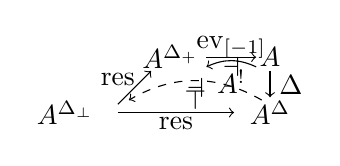
\begin{tikzpicture}[x=1.0em,y=1.0em]
  \node (B1) at (0,0) {$A^{\Delta_{\perp}}$};
  \node (T1) at (3.8,2.0) {$A^{\Delta_{+}}$};
  \node (T1R) at (7.4,2.0) {$A$};
  \node (R1) at (7.4,0) {$A^{\Delta}$};
  \draw[->] (1.9,0.3) -- (3.1,1.5);
  \node at (1.9,1.2) {$\mathrm{res}$};
  \draw[->] (5.1,2.0) -- (6.9,2.0);
  \node at (6.0,2.34) {$\mathrm{ev}_{[-1]}$};
  \node at (6.0,1.66) {$\dashv$};
  \draw[->] (6.9,1.65) to[bend right=25] node[below]{$A^{!}$} (5.1,1.65);
  \draw[->] (7.4,1.5) -- (7.4,0.55);
  \node at (8.15,1.0) {$\Delta$};
  \draw[->] (1.9,0) -- (6.1,0);
  \node at (4.0,-0.38) {$\mathrm{res}$};
  \draw[->,dashed] (7.1,0.45) to[bend right=30] node[below]{$\top$} (2.3,0.45);
  \node at (4.7,0.9) {$\dashv$};
\end{tikzpicture}
\end{center}
由附录 B 中的\cref{lem:absolute-lifting-under-adjunction}，这些\trAdjunction{}见证了：$[-1]$ 处的取值连同来自%
\cref{eq:nu-initial-transformation}的 2-\trCell{}，定义了典范限制\trFunctor{}
$A^{\Delta_{\perp}}\to A^{\Delta}$ 沿\trConstantFunctor{}的一个绝对右\trLifting{}，
如所断言。\trColimit{}的情形通过应用复合\trTwoFunctor{}
\begin{equation*}
\Cat^{\mathrm{coop}}
\xrightarrow{\ (-)^{\mathrm{op}}\ }\Cat^{\mathrm{op}}
\xrightarrow{\ A^{(-)}\ }\mathrm{h}\mathcal{K}
\end{equation*}
类似地证明。从附录 B 中的\cref{exa:top-splitting-adjunctions}出发的类似论证构造出顶部可裂（top splitting）
情形的绝对\trLifting{}图。

最后，由\trSimplicial\trCotensor{}的\trTwoFunctor{}性，任何\trFunctor{}
$f\colon A\to B$ 都与由 $\nu$ 或其对偶 $\nu^{\mathrm{op}}$ 作余张量所定义的
2-\trCell{}交换：
\begin{center}
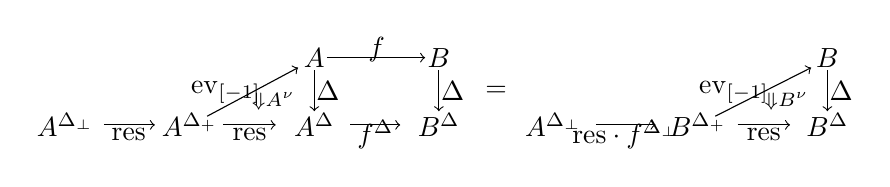
\begin{tikzpicture}[x=0.9em,y=0.9em]
  \node (B1) at (0,0) {$A^{\Delta_{\perp}}$};
  \node (B2) at (5.0,0) {$A^{\Delta_{+}}$};
  \node (B3) at (10.0,0) {$A^{\Delta}$};
  \node (B4) at (15.0,0) {$B^{\Delta}$};
  \node (TA) at (10.0,2.7) {$A$};
  \node (TB) at (15.0,2.7) {$B$};
  \draw[->] (1.55,0) -- (3.6,0);
  \node at (2.55,-0.4) {$\mathrm{res}$};
  \draw[->] (6.35,0) -- (8.45,0);
  \node at (7.4,-0.4) {$\mathrm{res}$};
  \draw[->] (11.45,0) -- (13.45,0);
  \node at (12.45,-0.4) {$f^{\Delta}$};
  \draw[->] (10.5,2.7) -- (14.45,2.7);
  \node at (12.5,3.04) {$f$};
  \draw[->] (10.0,2.2) -- (10.0,0.55);
  \node at (10.55,1.35) {$\Delta$};
  \draw[->] (15.0,2.2) -- (15.0,0.55);
  \node at (15.55,1.35) {$\Delta$};
  \draw[->] (5.7,0.35) -- (9.35,2.3);
  \node at (6.45,1.3) {$\mathrm{ev}_{[-1]}$};
  \node at (8.35,0.95) {$\scriptstyle\Downarrow A^{\nu}$};
  \node at (17.3,1.35) {$=$};
  \node (C1) at (19.6,0) {$A^{\Delta_{\perp}}$};
  \node (C2) at (25.4,0) {$B^{\Delta_{+}}$};
  \node (C3) at (30.6,0) {$B^{\Delta}$};
  \node (TB2) at (30.6,2.7) {$B$};
  \draw[->] (21.3,0) -- (23.7,0);
  \node at (22.5,-0.4) {$\mathrm{res}\cdot f^{\Delta_{\perp}}$};
  \draw[->] (27.0,0) -- (29.1,0);
  \node at (28.05,-0.4) {$\mathrm{res}$};
  \draw[->] (30.6,2.2) -- (30.6,0.55);
  \node at (31.15,1.35) {$\Delta$};
  \draw[->] (26.1,0.35) -- (29.95,2.3);
  \node at (26.85,1.3) {$\mathrm{ev}_{[-1]}$};
  \node at (28.95,0.95) {$\scriptstyle\Downarrow B^{\nu}$};
\end{tikzpicture}
\end{center}
由于右端的复合依\cref{lem:absolute-lifting-restriction}是绝对右\trLifting{}图，
左端的复合亦然；因此 $f\colon A\to B$ 保持 $A$ 中任何可裂余增广余单纯
对象的\trTotalization{}。
\end{proof}

\subsection*{练习}

\begin{exercise}\label{ex:ternary-products-from-binary}
证明：若∞-\trCategory{} $A$ 具有二元积，则它也具有三元积（事实上具有%
一切 $n\geq 1$ 的 $n$ 元积）。进一步证明：三元积\trFunctor{}可以由二元积%
\trFunctor{} $-\times-\colon A\times A\to A$ 出发定义为复合
$(-\times-)\times-$ 或复合 $-\times(-\times-)$；也就是说，证明这两个%
复合自然同构，且都满足刻画三元积的泛性质。
\end{exercise}

\begin{exercise}\label{ex:restriction-absolute-lifting}
证明\cref{lem:absolute-lifting-restriction}。
\end{exercise}

\begin{exercise}\label{ex:pasting-reproves-unit-counit}
用\trPastingDiagram{}计算重证\cref{lem:unit-counit-absolute-liftings}的%
正向蕴含，并类似地证明其逆向。
\end{exercise}

\begin{exercise}\label{ex:cospan-pullbacks}
设 $\CospanShape$ 为由两个箭头沿其余域粘合而成的\trCategory{}。形状为%
$\CospanShape$ 的\trDiagram{}称为\textbf{\trCospan}（cospan）。考虑把其中%
一支箭头送到恒同的满射\trFunctor{}
$\pi\colon\CospanShape\to\qcTwo$——这样的 $\pi$ 共有两个，任取其一。
证明：对任何∞-\trCategory{} $A$，相应的\trFunctor{}
$A^{\pi}\colon A^{\qcTwo}\to A^{\CospanShape}$ 容许穿过%
\trConstantFunctor{} $\Delta\colon A\to A^{\CospanShape}$ 的一个%
绝对右\trLifting{}。也就是说，证明任何∞-\trCategory{}都容许%
\trPullback{}，其中\trCospan{}的两支箭头之一是恒同。
\end{exercise}

\begin{exercise}[3.5.6]\label{ex:fully-faithful-liftings}
证明：对任何\trFunctor{} $f\colon A\to B$，恒同
\begin{center}
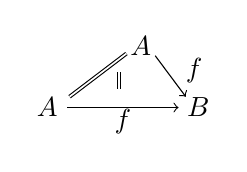
\begin{tikzpicture}[x=1.3em,y=1.3em]
  \node (At) at (2.6,1.7) {$A$};
  \node (Ab) at (0,0) {$A$};
  \node (Bb) at (4.2,0) {$B$};
  \draw[double] (0.62,0.3) -- (2.2,1.5);
  \draw[->] (3.0,1.44) -- (3.85,0.3);
  \node at (4.08,1.02) {$f$};
  \draw[->] (0.55,0) -- (3.65,0);
  \node at (2.1,-0.4) {$f$};
  \draw[double] (2.0,0.52) -- (2.0,1.0);
\end{tikzpicture}
\end{center}
定义 $f$ 穿过其自身的绝对\emph{右}\trLifting{}，当且仅当恒同定义 $f$
穿过其自身的绝对\emph{左}\trLifting{}；证法是逐一证明这两个条件都%
等价于如下断言：对任何∞-\trCategory{} $X$，诱导\trFunctor{}
$f_{\ast}\colon\mathrm{h}\Fun(X,A)\to\mathrm{h}\Fun(X,B)$
是\trFullyFaithful。\trFunctor{}之间「\trFullyFaithful」的第四种等价刻画见%
推论 3.5.6。
\end{exercise}

\begin{exercise}\label{ex:lifting-invariance-under-iso}
证明：与绝对右\trLifting{}图同构的图本身也是绝对右\trLifting{}图。
给定一个绝对右\trLifting{}图（左一）及自然同构
\begin{center}
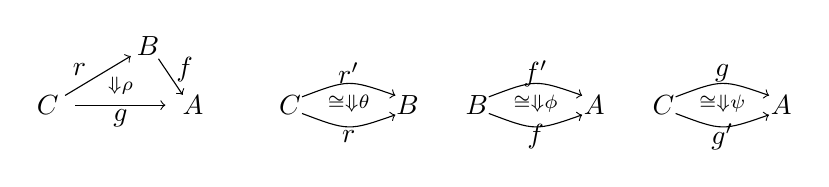
\begin{tikzpicture}[x=1.25em,y=1.25em]
  \node (C1) at (0,0) {$C$};
  \node (A1) at (4.2,0) {$A$};
  \node (B1) at (2.9,1.7) {$B$};
  \draw[->] (0.5,0.28) -- (2.4,1.42);
  \node at (0.92,1.02) {$r$};
  \draw[->] (3.2,1.34) -- (3.9,0.3);
  \node at (3.96,1.02) {$f$};
  \draw[->] (0.8,0) -- (3.4,0);
  \node at (2.1,-0.38) {$g$};
  \node at (2.1,0.55) {$\scriptstyle\Downarrow\rho$};
  \node (C2) at (7.0,0) {$C$};
  \node (B2) at (10.4,0) {$B$};
  \draw[->] (7.35,0.24) .. controls (8.7,0.75) .. (10.05,0.28);
  \node at (8.7,0.92) {$r'$};
  \draw[->] (7.35,-0.24) .. controls (8.7,-0.75) .. (10.05,-0.28);
  \node at (8.7,-0.92) {$r$};
  \node at (8.7,0.05) {$\scriptstyle\cong\Downarrow\theta$};
  \node (B3) at (12.4,0) {$B$};
  \node (A3) at (15.8,0) {$A$};
  \draw[->] (12.75,0.24) .. controls (14.1,0.75) .. (15.45,0.28);
  \node at (14.1,0.92) {$f'$};
  \draw[->] (12.75,-0.24) .. controls (14.1,-0.75) .. (15.45,-0.28);
  \node at (14.1,-0.92) {$f$};
  \node at (14.1,0.05) {$\scriptstyle\cong\Downarrow\phi$};
  \node (C4) at (17.8,0) {$C$};
  \node (A4) at (21.2,0) {$A$};
  \draw[->] (18.15,0.24) .. controls (19.5,0.75) .. (20.85,0.28);
  \node at (19.5,0.92) {$g$};
  \draw[->] (18.15,-0.24) .. controls (19.5,-0.75) .. (20.85,-0.28);
  \node at (19.5,-0.92) {$g'$};
  \node at (19.5,0.05) {$\scriptstyle\cong\Downarrow\psi$};
\end{tikzpicture}
\end{center}
证明粘贴所得的复合（下图）是一个绝对右\trLifting{}图。
\begin{center}
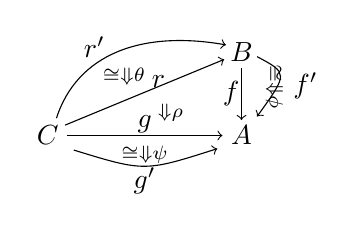
\begin{tikzpicture}[x=1.25em,y=1.25em]
  \node (C) at (0,0) {$C$};
  \node (B) at (5.6,2.4) {$B$};
  \node (A) at (5.6,0) {$A$};
  \draw[->] (0.25,0.5) .. controls (0.85,2.35) and (2.7,3.05) .. (5.15,2.62);
  \node at (1.35,2.55) {$r'$};
  \draw[->] (0.5,0.3) -- (5.1,2.2);
  \node at (3.2,1.55) {$r$};
  \node at (2.2,1.7) {$\scriptstyle\cong\Downarrow\theta$};
  \draw[->] (5.6,1.95) -- (5.6,0.45);
  \node at (5.3,1.2) {$f$};
  \draw[->] (6.05,2.28) .. controls (6.95,1.8) .. (6.05,0.55);
  \node at (7.45,1.45) {$f'$};
  \node[rotate=-90] at (6.55,1.4) {$\scriptstyle\cong\Downarrow\phi$};%
  \node at (3.55,0.66) {$\scriptstyle\Downarrow\rho$};
  \draw[->] (0.55,0) -- (5.05,0);
  \node at (2.8,0.34) {$g$};
  \draw[->] (0.75,-0.42) .. controls (2.8,-1.05) .. (4.9,-0.38);
  \node at (2.8,-0.55) {$\scriptstyle\cong\Downarrow\psi$};
  \node at (2.8,-1.3) {$g'$};
\end{tikzpicture}
\end{center}
由此推论：\trLimit{}与\trColimit{}在自然同构下不变。
\end{exercise}
